% Roll Number 13, Anjana Shankar S
.
\textbf{\textcolor{LightMagenta}{Distinguish between overfitting and underfitting. How it can affect model generalization? (September 2020 - Q3)
 \\. \hfill 4 marks}} \\[5pt]
 
\begin{tabular}{|p{7cm}|p{7cm}|}
    \hline
    \textcolor{purple}{Overfitting} & \textcolor{purple}{Underfitting}  \\ 
    \hline
    A statistical model is said to be overfitted, when we train it with a lot of data. & 
    A statistical model or a machine learning algorithm is said to have underfitting when it cannot capture the underlying trend of the data. \\
    \hline 
    
    When a model gets trained with lots of data it starts learning from the noise and inaccurate data entries in the data set. Then the model does not categorize the data correctly, because of too many details and noise. &
    Underfitting destroys the accuracy of the machine learning model. Its occurrence simply means that the model or the algorithm does not fit the data of too many details well enough.\\
    \hline
    
    The causes of overfitting are the non-parametric and non-linear methods because these types of Machine Learning algorithms have more freedom in building the model based on the dataset and hence they can really build unrealistic models. &
    It usually happens when we have less data to build an accurate model and also when we try to build a linear model with a non-linear data. In such cases, the rules of the machine learning model are too easy and flexible to be applied on such minimal data and therefore the model will probably make a lot of wrong predictions. \\
    \hline
    
    \hline
    A solution to avoid overfitting is using a linear algorithm if we have linear data or using the parameters like the maximal depth if we are using decision trees.& 
    Underfitting can be avoided by using more data and also reducing the features by feature selection\\
\hline
\end{tabular}

\begin{figure}[htp]
    \centering
    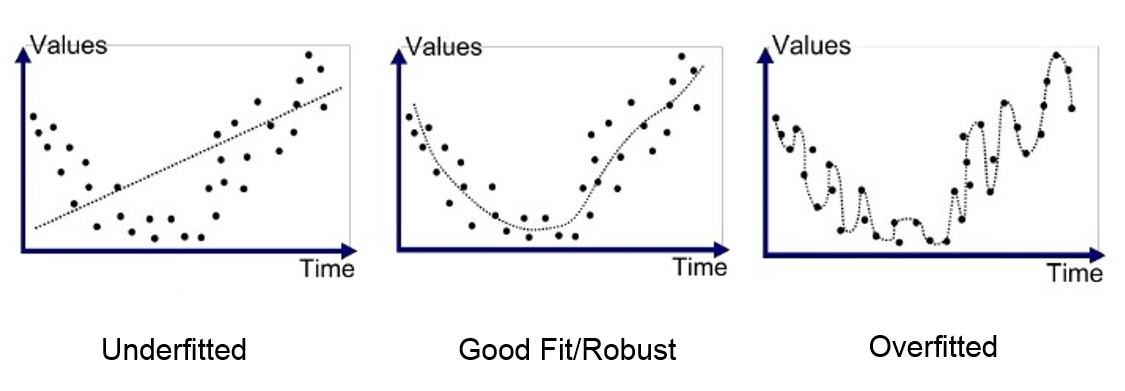
\includegraphics[width=10cm]{Images/A7_img1.png}
\end{figure}
\vspace{1cm}
  In terms of model generalization, in an overfitted model model generalization will be less. The model will have a tendency to give correct output only for those inputs which are present in the training dataset and give incorrect results to inputs not present in the dataset. On the other hand, an underfitted model shows very high model generalization causing it to give incorrect results to even an input present in the training dataset itself. 